\documentclass[t]{beamer}

% Load general definitions
% Preamble file - general definitions, package loading, etc.

%=================================
% Load packages
\usepackage{amssymb,amsmath}
\usepackage{graphicx}
\usepackage{url}
\usepackage{tikz}
\usetikzlibrary{mindmap,trees,arrows}
\usepackage{fancyvrb}
\usepackage[portuguese]{babel} 
\usepackage[utf8]{inputenc}
\usepackage{subfigure}
\usepackage{times}
\usepackage[T1]{fontenc}
\usepackage{cancel}
\usepackage{color}
\usepackage{listings}
\usepackage[document]{ragged2e}

%=================================
% Set mode
\mode<presentation>
{
	\usetheme{Madrid}
	\usecolortheme{structure}
	\useoutertheme{infolines}
	\setbeamercovered{invisible}
}

% Get rid of nav bar
\beamertemplatenavigationsymbolsempty

% Insert frame number at bottom of the page.
\usefoottemplate{\hfil\tiny{\color{black!90}\insertframenumber}} 

%=================================
% Define new commands

\newcommand\Real{{\mathbb{R}}}
%\newcommand{\vi}{\vspace{0.6\baselineskip}}
%\newcommand{\goodgap}{\hspace{\subfigtopskip}\hspace{\subfigbottomskip}}


% Equation environments
\newcommand{\beq}{\begin{equation}}
\newcommand{\eq}{\end{equation}}
\newcommand{\beqs}{\begin{equation*}}
\newcommand{\eqs}{\end{equation*}}
\newcommand{\beqn}{\begin{eqnarray}}
\newcommand{\eqn}{\end{eqnarray}}
% Bold variables
\newcommand{\mbf}[1]{\ensuremath{\mathbf{#1}}}
% Itemization
\newcommand{\bitem}{\begin{itemize}}
\newcommand{\eitem}{\end{itemize}}
\newcommand{\spitem}{\vskip 1em\item}
\newcommand{\bitems}{\begin{itemize}\item}
\newcommand{\benums}{\begin{enumerate}\item}
\newcommand{\eenum}{\end{enumerate}}
% color blocks
\newenvironment{colorblock}[2]{%
\setbeamercolor{block title}{#2}
\begin{block}{#1}}{\end{block}}
% Vertical spacing
\newcommand{\vone}{\vskip 1em}
\newcommand{\vhalf}{\vskip .5em}
% Frame environments
\newenvironment{ftst}[3][t]{%
\begin{frame}{environment=ftst,#1}
\frametitle{#2}
\framesubtitle{#3}}{\end{frame}}
\newenvironment{ftstf}[2]{
\begin{frame}[fragile,environment=ftstf]
\frametitle{#1}
\framesubtitle{#2}}{\end{frame}}
% colors
\definecolor{MyGray}{rgb}{0.5,0.5,0.5}
\definecolor{MyDBGray}{rgb}{0.1,0.1,0.4}
\definecolor{darkgreen}{rgb}{0,0.4,0}
\definecolor{black}{rgb}{0,0,0}
\def\defn#1{{\color{red} #1}}
% Footnote
\renewcommand{\thefootnote}{\alph{footnote}}
% Relaxed footnotes
\newcommand{\lfr}[1]{\let\thefootnote\relax\footnote{\tiny #1}}
% Verbatim environment - using FANCYVRB package
\DefineVerbatimEnvironment%
{rcode}{Verbatim}
{fontsize=\scriptsize}
% Verbatim environment - using LISTINGS package
%\lstnewenvironment{rcode} {\lstset{	language = R,
%									basicstyle = \scriptsize\ttfamily,
%									showspaces = false,
%									showstringspaces = false,
%									showtabs = false,
%									keywordstyle = \color{black}\bfseries,
%									commentstyle = \color{darkgreen},
%									numbers = none,
%									otherkeywords={	<-,
%													ggplot,
%													geom_boxplot,
%													facet_grid,
%													shapiro.test,
%													fligner.test,
%													glht,
%													with},
%									deletekeywords={data,
%													model,
%													residuals,
%													c,
%													axis,
%													default,
%													labels,
%													qq.text}}}%
%{}

% Specific definitions
\title[]{Metodologia Científica}
\subtitle[]{Apresentação de trabalhos científicos}
\author[]{Patrícia Lucas\\{\footnotesize }}
\institute{Bacharelado em Sistemas de Informação \\ IFNMG  - Campus Salinas}
\date{\scriptsize Salinas\\Julho 2021}

\begin{document}

% cover page
\setbeamertemplate{footline}{}
\begin{frame}

\begin{center}
\includegraphics[width=.15\textwidth]{}
\end{center}
  \titlepage
  \begin{tikzpicture}[remember picture,overlay]
  \node[anchor=south east,xshift=-5pt,yshift=5pt] at (current page.south east) {\tiny Versão 1.2021};
  \node[anchor=south west,yshift=0pt] at (current page.south west) {
\includegraphics[width=.25\textwidth]{Logos/salinas_horizontal_jpg.jpg}};
  \end{tikzpicture}  
\end{frame}

% Main slides
\begin{ftst}{Referência}{Preparação do texto}

\justifying
\begin{figure}
    \centering
    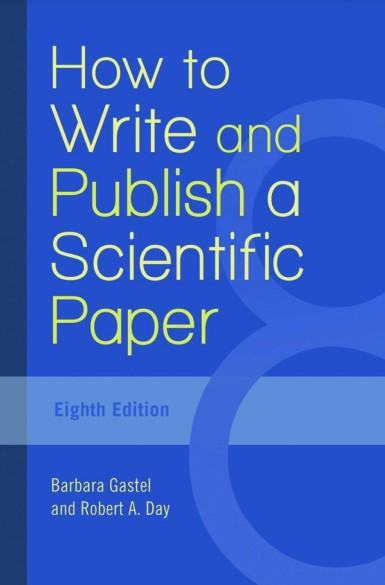
\includegraphics[scale=0.35]{Figuras/ref2.jpg}
\end{figure}

Gastel, Barbara; Day, Robert A. How to Write and Publish a Scientific Paper. Califórnia: Greenwood, 2016.

\end{ftst}
%=====

\begin{ftst}{Onde apresentar?}{Apresentação de trabalhos científicos}
\begin{itemize}
    \item O primeiro passo para apresentar um trabalho/artigo/resumo é obter a chance de fazê-lo.
    \vone
    \item Onde?
    \begin{itemize}
        \item Evento: oral ou pôster.
        \item TCC
    \end{itemize}
\end{itemize}
\end{ftst}

%=====

\begin{ftst}{Organização}{Apresentação de trabalhos científicos}
\begin{itemize}
    \item A melhor maneira de organizar um artigo para apresentação oral geralmente é proceder da mesma maneira lógica que se costuma fazer ao escrever um artigo.
    \item A apresentação oral não precisa e não deve conter todos os detalhes experimentais.
    \item A citação extensiva da literatura também é indesejável em uma apresentação oral.
\end{itemize}
\end{ftst}

%=====

\begin{ftst}{Organização}{Apresentação de trabalhos científicos}
\begin{itemize}
    \item A maioria das apresentações orais são curtas (com um limite de 10 minutos em muitas reuniões). 
    \item Assim, mesmo o conteúdo teórico deve ser reduzido em relação ao de um artigo escrito. Não importa o quão bem organizado seja, muitas ideias apresentadas muito rapidamente podem ser confusas. 
    \item Você deve se ater ao ponto ou resultado mais importante e enfatizá-lo. 
\end{itemize}
\end{ftst}

%=====

\begin{ftst}{Organização}{Apresentação de trabalhos científicos}
\begin{itemize}
    \item Existem, é claro, outros tipos mais longos de apresentações orais. 
    \item Um tempo típico alocado para apresentações de simpósios é de 20 minutos, seminários normalmente duram 1 hora. 
    \item Mesmo assim, você deve ir devagar, apresentando cuidadosamente alguns pontos ou temas principais. Se você avançar muito rápido, especialmente no início, seu público perderá o fio. 
    \item Os limites de tempo para apresentações em conferências tendem a ser rigorosamente cumpridos.
\end{itemize}
\end{ftst}

%=====

\begin{ftst}{Organização}{Apresentação de trabalhos científicos}
\begin{itemize}
    \item Planeje cuidadosamente sua apresentação para caber no tempo alocado. 
    \item Se possível, torne sua apresentação um pouco curta (digamos, 9 ou 9,5 minutos se houver 10 minutos), para acomodar lentidão inesperada. 
    \item Ensaie a sua apresentação com antecedência, tanto para se certificar de que tem o comprimento certo quanto para ajudar a garantir uma apresentação tranquila. 
\end{itemize}
\end{ftst}

%=====

\begin{ftst}{Dicas}{Apresentação de trabalhos científicos}
\begin{itemize}
    \item Fale muito claramente e evite falar rápido.
    \item Lembre-se de olhar para o público. 
    \item Mostre interesse em seu assunto. 
    \item Evite hábitos que possam distraí-lo.
    \item Para polir sua apresentação, considere gravar os ensaios em vídeo de uma ou mais de suas apresentações. 
    \item Esconda os sinais físicos de ansiedade. Por exemplo, se suas mãos tremem sob pressão, não segure um apontador laser. 
    \item Perceba que uma apresentação não precisa ser perfeita para ser excelente. Talvez o mais importante, perceba que os membros da audiência estão lá não porque desejam julgar seu estilo de falar, mas porque estão interessados em sua pesquisa.
\end{itemize}
\end{ftst}

%=====

\begin{ftst}{Slides}{Apresentação de trabalhos científicos}
\begin{itemize}
    \item Os slides devem ser projetados especificamente para uso em apresentações orais, com letras grandes o suficiente para serem vistos do fundo da sala.
    \item Em geral, use letras que tenham pelo menos tamanho 28. Escolha uma fonte sem serifa, como Arial ou Calibri.
    \item Elementos como figuras, gráficos e tabelas devem ser legíveis!
    \item Os slides não devem estar lotados. Cada slide deve ilustrar um ponto específico ou talvez resumir alguns.
    \item Para permitir uma leitura rápida, use marcadores, não parágrafos.
    \item Cuidado para não mostrar muitos slides. Um número moderado de slides bem escolhidos irá aprimorar sua apresentação; muitos distraem. 
    \item Uma diretriz geral é não exceder a média de cerca de um slide por minuto.
\end{itemize}
\end{ftst}

%=====

\begin{ftst}{Slides}{Apresentação de trabalhos científicos}
\begin{itemize}
    \item Caso resolva usar um apontador laser para chamar a atenção para um item específico em um slide, direcione o apontador especificamente para o item. Não gesticule descontroladamente para o slide ou para o público.
    \item O slide deve complementar o que você está dizendo e não simplesmente repetir o que você está dizendo.
    \item Slide de agradecimento: você pode incluir um slide de encerramento reconhecendo os colaboradores e talvez mostrando uma foto do grupo de pesquisa. 
    \item Slides cuidadosamente projetados, bem preparados e usados com habilidade podem aumentar muito o valor de uma apresentação científica.
\end{itemize}
\end{ftst}

%=====

\begin{ftst}{Como organizar o tempo?}{Apresentação de trabalhos científicos}
Apresentação de 30 minutos:
\begin{itemize}
    \item Treine a apresentação por partes primeiro para verificar os tempos de cada seção.
    \item Prepare uma apresentação mais curta: aqui coloquei 26 min.
\end{itemize}
\vone

\begin{figure}
    \centering
    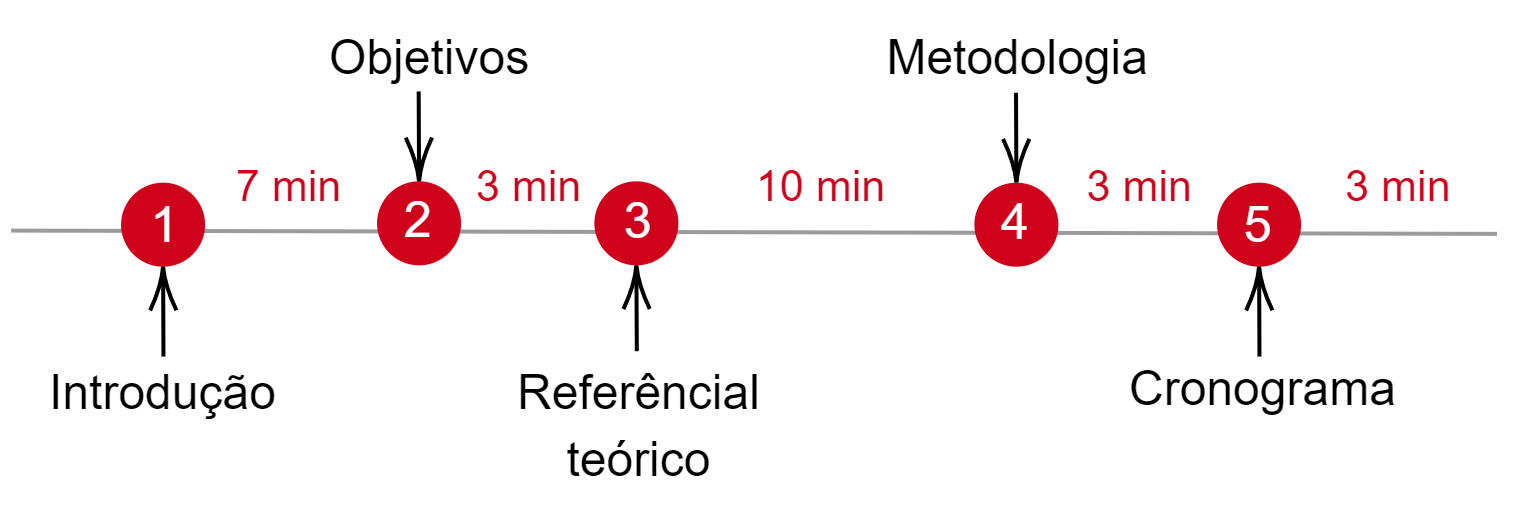
\includegraphics[scale=0.2]{Figuras/tempo.png}
\end{figure}
\end{ftst}

%=====

\begin{ftst}{\LARGE Último aprendizado da disciplina!}{=)}


\begin{figure}
    \centering
    
\includegraphics[scale=0.8]{Figuras/meme.jpeg}
\end{figure}
\end{ftst}

\end{document}